\documentclass[a4paper,UTF8,fontset = windowsnew]{ctexbook}
\usepackage[user=teacher]{cexam}
\usepackage[margin=2cm]{geometry}
%\usepackage[utf8]{inputenc}
%\usepackage{amsfonts}
%\usepackage{amssymb}
%\usepackage{amsmath}
%\usepackage{float}
\usepackage{tikz}
%\usetikzlibrary{patterns}
%\usepackage[european,oldvoltagedirection]{circuitikz}
%\usepackage{graphicx}
%\usepackage[
%  pdfborder=0 0 0,
%  bookmarksnumbered=true
%]{hyperref}
%\usepackage{draftwatermark}
%\usepackage{l3color}
%\usepackage{l3draw}
%\SetWatermarkText{冯振华手稿}
%\includeonly{
%   chapter-运动的描述,
%}

\begin{document}
\title{高中物理讲义}
\author{冯振华}
\date{2019年9月1日}
%\maketitle
%\frontmatter
%\tableofcontents

%  \chapter{运动的描述}
  \section{运动学基本概念}
\subsubsection{质点}

在研究物体的机械运动时,为简化问题可以抓住主要问题忽略次要问题做一定的简化.如果在所研究的问题中,物体的\CJKunderwave{大小和形状对该问题影响不大}时,则可以忽略物体的大小,将物体看成一个有质量的几何点,叫做质点.

质点是一种\CJKunderwave{理想物理模型},它实际上不存在,由于问题的复杂性往往采用一定的近似使它简化.比如,点电荷也是一种理想模型,还有理想变压器等.

\begin{selection}
  s1.下列关于质点的说法中,正确的是[D]
  A.质点是一个理想化的模型,实际上并不存在,所以引入这个概念没有多大意义
  B.体积很小的物体更容易看做质点
  C.凡轻小的物体,皆可看做质点
  D.当物体的形状和大小对所研究的问题属于无关或者次要因素时,即可把物体看成质点

  a.*

  e.建立理想模型是物理中的重要的研究方法,对于复杂问题的研究有重大意义,A错误;一个物体能否看做质点不应看其大小,关键是看其大小对于研究的问题的影响能否忽略,体积很小的物体有时可以看成质点,有时不能看成质点,B错误;一个物体能否看成质点不以轻重而论,C错误;物体能否看成质点取决于其大小和形状对所研究的问题是否属于无关或次要因素,若是就可以看成质点,D正确.

\end{selection}
\subsubsection{参考系}
要描述一个物体的运动,首先要选定某个其它的物体做参考,观察物体相对于这个``其它物体''的位置是否随时间变化,以及怎样变化.这种 \CJKunderwave{用来做参考的物体} 称为参考系.

对一个物体的运动情况的描述,取决于所选择的参考系,选取的参考系不同,对于同一个物体运动的描述一般也不相同.

参考系具有相对性.它的具体含意为:对于一个物体的运动, \CJKunderwave{总能够找到一个参考系,使该物体对于此参考系是静止的} ,也就是静止具有相对性.对于多个物体,一般它们的运动不相同, \CJKunderwave{找不到一个参考系,使所有的物体对于该参考系都静止} ,也就是运动具有绝对性.

\begin{selection}
  s1.关于参考系,下列说法正确的是[D]
  A.参考系必须是静止不动的物体
  B.参考系必须是静止不动或正在做直线运动的物体
  C.研究物体的运动,可选择不同的参考系,但是选择不同的参考系观察的结果是一样的
  D.研究物体的运动,可选择不同的参考系,但选择不同的参考系研究同一物体的运动而言,一般会出现不同的结果

  a.*

  e.参考系的选取是任意的,A,B错误;选择不同的参考系,对同一物体运动的描述一般是不同的,C错误,D正确.

\end{selection}

\subsubsection{坐标系}
上一节中,参考系可以确定物体是静还是动的问题.但是不能确定动多么快的问题,也就是定性的,所以要准确的描述物体的位置及位置变化需要建立坐标系,这个坐标系包括:\CJKunderwave{原点,正方向和单位长度.}

研究物体的直线运动时,一般建立直线坐标系,研究物体的曲线运动(轨迹是曲线的运动)时建立平面直角坐标系.另外还有极坐标系,自然坐标系等.感兴趣的同学可以参考一下相关的数学资料.\CJKunderwave{所有坐标系中的一个点和物体的位置一一对应}.

\begin{calculate}
c1.一质点在x轴上运动,各个时刻的位置坐标如
<:
\begin{tabular}{|*{7}{c|}}
  \hline
  t/s & 0 & 1 & 2 & 3 & 4 & 5\\
  \hline
  x/m & 0 & 5 & -4 & -1 & -7 & 1\\
  \hline
\end{tabular}
:>所示:
[1]请画出x轴,在上面标出质点在各个时刻的位置.
[2]哪个时刻离开坐标原点最远?有多远?

a.见解析

e.(1)各时刻质点的位置坐标如
<:
{\tiny	
  \begin{tikzpicture}[scale=0.4]
    \draw [->] (-8,0)--(7,0);
    \foreach \x in {-7,-6,-5,-4,-3,-2,-1,0,1,2,3,4,5}
    \draw (\x,0pt)--(\x,3pt) node [anchor=north] {\x};
    \draw (8,0) node [anchor=north east] {$x/m$};
    \draw [<-] (-7,4pt)--(-7,24pt) node [anchor=south]{ 4s 末};
    \draw [<-] (-4,4pt)--(-4,24pt) node [anchor=south]{ 2s 末};
    \draw [<-] (-1,4pt)--(-1,24pt) node [anchor=south]{ 3s 末};
    \draw [<-] (1,4pt)--(1,24pt) node [anchor=south]{ 5s 末};
    \draw [<-] (5,4pt)--(5,24pt) node [anchor=south]{ 1s 末};
    \draw [<-] (0,4pt)--(0,44pt) node [anchor=south]{0时刻};
  \end{tikzpicture}
}
:>所示.
\newline
(2)由图可知第4s 末质点离开坐标原点最远,有7m.


\end{calculate}

\subsubsection{时刻}

时刻指的是\CJKunderwave{某一瞬间},在时间轴上\CJKunderwave{时刻用点表示}.

\subsubsection{时间间隔}

时间间隔指某两个时刻之间的间隔,在时间轴上用\CJKunderwave{线段}来表示.

\begin{selection}
  s1.以下计时数据指时间间隔的是[B]
  A.天津开往德州的 k625 次列车于13 点35分从天津发车
  B.李明用15s跑完100米
  C.2013年6月11日下午17时38分,``神舟十号'' 飞船成功发射
  D.某场足球开赛15分钟时甲队攻入一球

  a.B

  e. 列车发车、飞船发射、入球都是事件发生的瞬间,对应的都是时刻,A、C、D错误;跑完100m 是事件发生的过程,对应的是时间间隔,B正确。

\end{selection}

\subsubsection{矢量和标量}
在物理学中,根据不同的物理量的性质可以分为两类:一类\CJKunderwave{既有大小又有方向},同时运算满足\CJKunderwave{平行四边形定则}的称为矢量;另一类是\CJKunderwave{只有大小没有方向},其运算遵守\CJKunderwave{代数运算},称为标量.

平行四边形定则如下:

\begin{figure}[H]
  \centering
  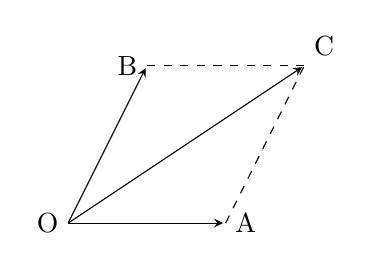
\begin{tikzpicture}
    \draw [->,>=stealth,shorten >=1pt] (0,0)--(2,0) node [anchor=west]{A};
    \draw [->,>=stealth,shorten >=1pt] (0,0)--(1,2) node [anchor=east]{B};
    \draw [dashed] (1,2) --(3,2);
    \draw [dashed] (2,0)--(3,2);
    \draw [->,>=stealth,shorten >=1pt] (0,0)--(3,2) node [anchor=south west]{C};
    \draw (0,0) node [anchor=east]{O};
  \end{tikzpicture}
  \caption{平行四边形定则}
  \label{fig:parallelogram law}
\end{figure}

$$\vec{C}=\vec{A}+\vec{B}$$

数学上舍弃矢量的实际含义,就抽象为数学中的概念---向量.同学们要掌握向量的计算方法,如果不熟悉的话,请参考数学书籍先补充上这一部分知识.

\subsubsection{路程}

路程指\CJKunderwave{物体运动轨迹的长度},是一个\CJKunderwave{标量}.

\subsubsection{位移}

位移指从\CJKunderwave{初位置}到\CJKunderwave{末位置}的有向线段,是一个矢量,大小就是该有向线段的长度,方向就是前头所指的方向.

描述一个物体的机械运动,准确的应该使用位移.但是同学们在读初中的时候使用路程来计算,并没有遇到错误,那是因为在初中研究的都是单向直线运动,\CJKunderwave{单向直线运动中位移的大小与路程相等},同时只有一个方向,所以在计算过程中略去方向的考虑并不会导致问题.

\begin{figure}[H]
  \centering
  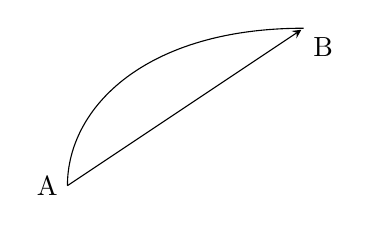
\begin{tikzpicture}
    \draw (0,0) .. controls (0,1) and (1,2) .. (3,2);
    \draw [->,>=stealth,shorten >=1pt] (0,0) -- (3,2);
    \draw (0,0) node [anchor=east]{A};
    \draw (3,2) node [anchor=north west]{B};
  \end{tikzpicture}
  \caption{位移}
  \label{fig:displacement}
\end{figure}

如图\ref{fig:displacement}所示,由A到B的位移记为$\overrightarrow{AB}$,但是路程由两个不同的路径是不同的.同时也能看到,对于\CJKunderwave{曲线运动它的位移大小小于路程},但是单向直线运动中它们是相等的.

对于直线运动的位移可以用$x_1$表示质点的起始位置,$x_2$表示质点的末位置,则以$\Delta x=x_2-x_1$表示位移.
如果$\Delta x>0$表示位移方向向右,如果$\Delta x<0$表示位移方向向左.

\begin{figure}[H]
  \centering
    \begin{tikzpicture}
      \draw [->] (0,0)--(3,0) node [anchor=north] {\small $x/m$};
      \draw (1,0)--(1,4pt) node [anchor=south] {\small $x_1$};
      \draw (2,0)--(2,4pt) node [anchor=south] {\small $x_2$};
    \end{tikzpicture}
  \caption{直线运动的位移}
\end{figure}

  \begin{selection}
    s1.下列关于位移(矢量)和温度(标量)的说法中,正确的是[D]
    A.两个运动物体的位移大小均为$30m$,则这两个位移一定相同
    B.做直线运动的两个物体的位移$x_1=3m$, $x_2=-5m$,则$x_1>x_2$
    C.温度计计数有正也有负,其正,负号表示方向
    D.温度计计数的正负号表示温度的高低,不能表示方向

    a.*

    e.两个矢量相同指矢量的大小和方向两个要素都相同,所以A由于可能方向不同,所以错;直线运动的位移的``$+$''表示与正方向相同,``$-$''表示与正方向相反;温度是标量,标量的正负号表示大小(也就是温度的高低).

    s2.(多选)关于位移和路程,下列说法正确的是[BCD]
    A.在某一段时间内物体运动的位移为零,则该物体一定是静止的
    B.在某一段时间内物体运动的路程为零,则该物体一定是静止的.
    C.在直线运动中,物体的位移大小可能等于其路程
    D.在曲线运动中,物体的位移大小一定小于其路程

    a.BCD

    e.位移为零,表明该物体在运动过程中的初、末位置相同,物体不一定静止,A项错误;路程为零,表明运动轨迹的长度为零,物体一定静止,B项正确;当物体做单向直线运动时,其位移大小等于路程,C项正确;物体在做曲线运动时,初、末位置直线距离小于轨迹长度,所以位移大小一定小于路程,D项正确.

    s3.(多选)对位移和路程理解正确的是[BC]
    A.路程是个标量,是由初始位置指向终止位置的有向线段
    B.位移是个矢量,是由初始位置指向终止位置的有向线段
    C.路程是物体实际运动轨迹的长度,它没有方向
    D.当物体做直线运动时,位移和路程是相同的物理量

    a.BC

    e.路程是物体实际运动轨迹的长度,是标量;位移是由初始位置指向终止位置的有向线段,是矢量.当物体做单向直线运动时,两者大小相等,但不相同.综上,选项B,C正确.

  \end{selection}
  \begin{calculate}
   c1.如
   <:
   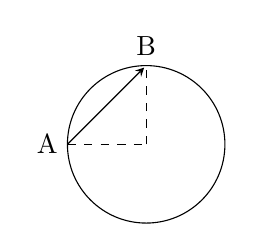
\begin{tikzpicture}
     \draw (0,0) circle [radius=1];
     \draw [->,>=stealth,shorten >=1pt] (-1,0) --(0,1);
     \draw (-1,0) node [anchor=east]{A};
     \draw (0,1) node [anchor=south]{B};
     \draw [dashed] (0,0) --(0,1);
     \draw [dashed] (-1,0)--(0,0);
   \end{tikzpicture}
   :>
   所示,一质点沿半径为$20cm$ 的圆周自A 点出发,逆时针运动$\cfrac{3}{4}$圆周到达B点.求质点的位移和路程.

a. 位移大小为$28.3cm$,方向自A点指向B点,路程为$94.2cm$

e.如图,位移大小为AB线段的长度
$$AB=\sqrt{2}r\approx28.3cm$$
方向:由A点指向B点
\newline
路程为
$$s=\cfrac{3}{4}\cdot2\pi r=94.2cm$$

c2.一个袋子里有$40kg$ 大米,再放入$30kg$大米,袋子中大米的质量是多少?如果一位同学从操场中心A点出发向北走了$40m$ 到达B点,然后又向西走了$30m$ 到达C点,则他从A点到C点的路程是多大?位移是多少?从大小的计算方法上看,质量、路程和位移有什么不同?

a.见解析

e.袋子中大米的质量是$40kg+30kg=70kg$.如
<:
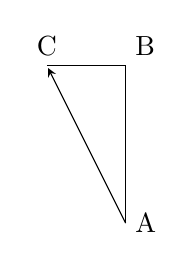
\begin{tikzpicture}
  \draw [->,>=stealth,shorten >=1pt] (0,0)--(-1,2) node [anchor=south]{C};
  \draw (0,0) -- (0,2) node [anchor=south west]{B};
  \draw (-1,2)--(0,2);
  \draw (0,0) node [anchor=west]{A};
\end{tikzpicture}
:>所示,路程是$40m+30m=70m$,位移从A点指向C点的有向线段,大小为$AC=50m$.质量,路程是标量,遵从算术加减法的法则,可以直接相加减;位移是矢量,不能直接相加减,位移的大小等于初位置指向末位置的有向线段的长度.

  \end{calculate}


  \newpage
  \section{速度和速率}
\subsection{机械运动}
物体的位置随时间的变化,我们称之为机械运动.简言之,就是研究物体的位移随时间的变化.
\subsection{速度}
\subsubsection{定义}
质点在$\Delta t$ 时间内发生的位移$ \Delta x $ 与 时间的比值,定义为速度.用公式表达如下
\begin{equation}
  v=\cfrac{\Delta x}{\Delta t}\label{eq:velocity}
\end{equation}
\subsubsection{矢标性}
 从定义上来看,位移$\Delta x$ 是一个矢量,时间$\Delta t$ 是一个标量,矢量除以标量还是一个矢量.所以速度是一个矢量.速度的方向我们称之为质点运动的方向,在一些题目中没有明确提出,也这样认为.
 \subsubsection{单位}
 每一个物理量都有一个特定的意义,所以也必然有一个单位.从定义看来,位移的单位是``米'',时间的单位是``秒'',所以速度单位是:米/秒,符号为$m/s$
\subsubsection{速度的物理意义}
速度是表征物体运动快慢的物理量.这里大家注意,如果问某个物理量的物理意义,我们统一的说法是:XX是表征XXXX的物理量.
\subsection{瞬时速度和平均速度}
\subsubsection{瞬时速度}
瞬时速度描述物理某一瞬时的运动的快慢,所以要求时间$\Delta t \rightarrow 0$,瞬时速度的定义为:
\begin{equation}
 v=\lim_{\Delta t \to 0} \cfrac{\Delta x}{\Delta t}
  \label{eq:instantaneous velocity}
\end{equation}

\subsubsection{平均速度}
平均速度描述质点运动的平均快慢程度,所以是在一段时间内发生的,不要求时间趋于零.为了区别于瞬时速度,在速度$v$ 的上方加一个横杠$\overline{v}$,读作 ``维拔'',其定义为:
\begin{equation}
\overline{v}=\cfrac{\Delta x}{\Delta t}
  \label{eq:average velocity}
\end{equation}

\subsection{速率}
\subsubsection{定义}
速率是指路程比上时间,表示单位时间内发生的路程.定义如下
\begin{equation}
v=\cfrac{\Delta s}{\Delta t}
  \label{eq:speed}
\end{equation}

\subsubsection{矢标性}
从速率的定义来看,路程是标量,时间是标量,所以速率也是一个标量.

\subsubsection{单位}
从速率定义来看,速率的单位和速度相同,都是$m/s$



\subsubsection{瞬时速率}
类比速度,则速率也分为瞬时速率和平均速率,瞬时速率定义如下:
\begin{equation}
v=\lim_{\Delta t \to 0} \cfrac{\Delta s}{\Delta t}
  \label{eq:instantaneous speed}
\end{equation}

\subsubsection{平均速率}
类比速度,则速率也分为瞬时速率和平均速率,平均速率定义如下:
\begin{equation}
\overline{v}=\cfrac{\Delta s}{\Delta t}
  \label{eq:average speed}
\end{equation}

\subsubsection{注意事项}
在初中时同学们运算都采用的速率,但是当时没有区分速度和速率,因为当时研究的是单向直线运动,这种情况下速度的大小和速率是相等的,所以没有出现错误.然而一旦情况复杂,则必须用速度来描述.

今后如没有特殊声明,则一律使用速度来描述运动,不再使用速率.

\subsection{例题分析}
\begin{selection}
  1.关于速度的定义$v=\frac{\Delta x}{\Delta t}$ ,以下叙述正确的是
  A.物体做匀速直线运动时,速度$v$ 与运动的位移 $\Delta x$ 成正比,与运动时间$\Delta t$ 成反比
  B.速度$v$ 的大小与运动的位移$\Delta x$ 和时间$\Delta t$ 都无关
  C.此速度定义适用于任何运动
  D.速度是表示物体运动快慢及方向的物理量

  a.BCD

  e.$v=\frac{\Delta v}{\Delta t}$ 是速度的定义式,所以适用于一切情况,C对;此定义法为比值定义法,不能说此物理量与分子成正比或者与分母成反比,所以A错,B对;速度的大小表示运动的快慢,方向表示物体运动的方向,所以D对.

  2.物体沿直线做单向直线运动,途经直线上的A,B,C 三点,经过这三点时的速度分别为$v_A$ , $v_B$ , $v_C$ ,则下列说法正确的是
  A.$v_A$, $v_B$ , $v_C$ 越大,则由A到C所用的时间越短
  B.经过 A,B,C 三点时的瞬时速率就是$v_A$ , $v_B$ , $v_C$
  C.由A到C这一阶段的平均速度为$\overline{v}=\frac{v_A+v_B+v_C}{3}$
  D.由A到C这一阶段的平均速度越大,则由A到C所用的时间越短

  a.D

  e.A到C所用时间取决于A到C的平均速度,与初,末态的瞬时速度无关,A错误,D正确.瞬时速度的大小叫瞬时速率,B错误.平均速度一般不等于速度的平均值,C错误.

\end{selection}

\begin{calculate}
3.一辆汽车由A出发做直线运动,前$5s$ 向东行驶了$30m$ 到达 B 点,又行驶了$5s$ 前进了$60m$ 到达 C点,在C点停了$4s$ 后又向西行驶,经历了$6s$  运动$12m$ 到达 A点西侧的D点.求
[1]全过程的平均速度;
[2]全过程的平均速率.

a.(1)平均速度大小为$1.5m/s$,方向水平向西 (2) 平均速率为$10.5m/s$

e.(1)设向东为正方向
$$x=30m+60m+(-120m)=-30m$$
全程用时
$$t=5s+5s+4s+6s=20s$$
所以平均速度为
$$\overline{v}=\cfrac{x}{t}=\cfrac{-30m}{20s}=-1.5m/s$$
负号表示速度方向向西
\newline
(2)全程的路程为
$$s=30m+60m+120m=210m$$
所以平均速率为
$$\overline{v}=\cfrac{s}{t}=\cfrac{210m}{20s}=10.5m/s$$


\end{calculate}

  \newpage
  \section{加速度}
在描述物体的机械运动时,我们不仅要知道某一时刻物体在哪里(位移),向哪个方向运动的快慢(速度),而且也需要知道\CJKunderwave{物体速度变化的快慢},所以引入加速度.

\subsection{加速度}
\subsubsection{定义}
加速度定义为\CJKunderwave{速度的变化量}和\CJKunderwave{时间}的比值,如下
\begin{equation}
  a=\cfrac{\Delta v}{\Delta t} \label{eq:acceleration}
\end{equation}

\subsubsection{物理意义}
\CJKunderwave{加速度}是表征物体\CJKunderwave{速度变化快慢}的物理量.

\subsubsection{矢标性}
从定义上来看,速度的变化量$\Delta v$ 是矢量,时间 $\Delta t$ 是标量,所以加速度也是一个\CJKunderwave{矢量}.它的方向与\CJKunderwave{速度变化量}$\Delta v$ 的方向一致.
\subsubsection{单位}
从定义上来看,速度变化量的单位是$m/s$,时间的单位是$s$ ,所以加速度的单位是:\CJKunderwave{ 米每二次方秒},记作$m/s^2$

\subsection{瞬时加速度和平均加速度}
类比瞬时速度和平均速度,加速度也有瞬时加速度和平均加速度.

\subsubsection{瞬时加速度}
瞬时加速度用来描述某\CJKunderwave{一个时刻}速度变化的快慢.其定义如下:
\begin{equation}
a=\lim_{\Delta t \to 0} \cfrac{\Delta v}{\Delta t}
  \label{eq:instantaneous acceleration}
\end{equation}

\subsubsection{平均加速度}
平均加速度用来描述某\CJKunderwave{一段时间}内速度平均变化快慢.其定义如下:
\begin{equation}
\overline{a} =\cfrac{\Delta v }{\Delta t}
  \label{eq:average acceleration}
\end{equation}

\subsection{加速与减速的判断}

在具体的运动中,物体有可能加速也有可能减速,但是没有{\bf 减速度}一词.所有变速运动速度的变化量与
时间的比值都叫加速度,这只是一个名称而已.

如果物体运动的轨迹是直线,则称为直线运动,在直线运动中,如果 $v$ 与 $a$ 方向相同则加速,如果 $v$ 与 $a$ 的方向相反则减速.

如果物体运动的轨迹是曲线,则称为曲线运动,在曲线运动中,如果 $v$ 与 $a$ 的夹角是锐角则加速,如果 $v$ 与 $a$ 夹角为钝角则减速,如果 $v$ 与 $a$ 的夹角是直角,则速度大小不发生变化,只有速度的方向发生变化.

\subsection{注意事项}
在物理学中经常用比值定义法来定义物理量,这就好比用钱来定义钱包一样:\CJKunderwave{钱包是用来盛钱的包}.但是钱包和钱的多少没关系.所以加速度$a$ 和 $\Delta v$也没有关系,与$\Delta t$也没有关系,它\CJKunderwave{只取决于速度变化量和时间的比值}.

$\Delta$这个符号用来表示\CJKunderwave{一个末态的量减去一个初态的量},比如:$\Delta v =v_2 -v_1$,其中$v_1$是初始的速度,$v_2$是末速度.以后遇到的所有$\Delta$都具备此含义.

按上面的表述,则$\Delta t >0$是\CJKunderwave{永远成立}的.所以$a$与$\Delta v$的符号相同,因此说加速度的方向与速度变化量的方向一致.

\subsection{例题分析}
\begin{selection}
  1.一辆汽车正在公路上行驶,关于汽车的运动,下列说法正确的是
  A.汽车的速度改变量越大,加速度一定越大
  B.速度很大的汽车,其加速度可能很小,但不能为零
  C.某时刻汽车的速度为零,其加速度可能很大
  D.汽车加速度很大时,其速度一定很大

  a.C

  e.汽车的速度改变量越大,加速度不一定越大,因为加速度与速度改变量和时间间隔两个因素有关,选项A错误;速度很大的汽车,加速度可能很小,也可能为零,例如匀速直线运动的汽车,选项B 错误;汽车速度为零时,加速度可能很大,例如汽车刚启动时,选项C正确,D错误.

  2.由加速度的定义式$a=\cfrac{\Delta v}{\Delta t}$可知
  A.加速度$a$与速度的变化$\Delta v$ 成正比
  B.加速度$a$ 大小由速度变化$\Delta v$ 决定
  C.加速度$a$ 的方向与速度$v$ 的方向 相同
  D.加速度$a$ 的方向与$\Delta v$的方向相同

  a.D

  e.$a=\cfrac{\Delta v}{\Delta t} $ 是加速度的定义式,是比值定义法,不能说加速度与分子和分母单独有关,所以A,B 错误.由于$\Delta t>0$ 永远成立,所以 $a$ 的符号与$\Delta v$ 的正负号相同,一个矢量正负号表示方向,所以D 正确.

  3.某物体沿直线运动,其$v-t$ 图象如
  <:
  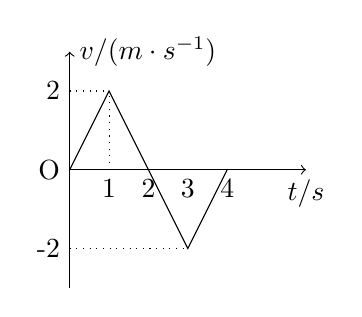
\begin{tikzpicture}
    \draw[->] (0,0)--(3,0) node [anchor=north ]{$t/s$};
    \draw[->] (0,-1.5)--(0,1.5) node [anchor=west]{$v/(m\cdot s^{-1})$};
    \draw (0,0) node [anchor=east] {O};
    \draw (0.5,0) node [anchor=north]{1};
    \draw (1,0) node [anchor=north]{2};
    \draw (1.5,0) node [anchor=north]{3};
    \draw (2,0) node [anchor=north]{4};
    \draw (0,0)--(0.5,1)--(1.5,-1)--(2,0);
    \draw [dotted](0,1)node [anchor=east]{2}--(0.5,1);
    \draw [dotted] (0.5,0)--(0.5,1);
    \draw [dotted](0,-1)node [anchor=east]{-2}--(1.5,-1);
  \end{tikzpicture}
  :>所示,下列说法正确的是
  A.第$1s$ 内和 第$2s$ 内物体的速度方向相反
  B.第$1s$ 内和第$2s$ 内物体的加速度方向相反
  C.第$3s$ 内物体的速度方向和加速度方向相反
  D.第$2s$ 末物体的加速度为零

  a.B

  e.速度的方向由纵坐标的正负表示,正号表示与正方向相同,负号表示与正方向相反.加速度的方向由$v-t$ 图象的斜率的正负表示,正号表示加速度沿正方向,负号表示加速度沿负方向.第$1s$ 内,第$2s$ 内纵坐标为正,速度均为正向,A错误;根据斜率的正负,第$1s$ 内加速度为正向,第$2s$ 内加速度为负方向,B正确;第$3s$ 内速度为负方向,加速度为负方向,C错误;第$2s$ 末物体的加速度为$-2m/s^2$,D错误.

\end{selection}


\chapter{运动的描述}
\section{运动学基本概念}

\subsection{坐标系}
上一节中,参考系可以确定物体是静还是动的问题.但是不能确定动多么快的问题,也就是定性的,所以要准确的描述物体的位置及位置变化需要建立坐标系,这个坐标系包括:\CJKunderwave{原点,正方向和单位长度.}

研究物体的直线运动时,一般建立直线坐标系,研究物体的曲线运动(轨迹是曲线的运动)时建立平面直角坐标系.另外还有极坐标系,自然坐标系等.感兴趣的同学可以参考一下相关的数学资料.\CJKunderwave{所有坐标系中的一个点和物体的位置一一对应}.

\begin{jisuan}[example]
   1.一质点在x轴上运动,各个时刻的位置坐标如
   \begin{tabular}{|*{7}{c|}}
      \hline
      t/s & 0 & 1 & 2 & 3 & 4 & 5\\
      \hline
      x/m & 0 & 5 & -4 & -1 & -7 & 1\\
      \hline
   \end{tabular}
   所示:
   \qitem 请画出x轴,在上面标出质点在各个时刻的位置.
   \qitem 哪个时刻离开坐标原点最远?有多远?

   a.见解析

   e.(1)各时刻质点的位置坐标如
      \begin{tikzpicture}[scale=0.4]
	 \draw [->] (-8,0)--(7,0);
	 \foreach \x in {-7,-6,-5,-4,-3,-2,-1,0,1,2,3,4,5}
	 \draw (\x,0pt)--(\x,3pt) node [anchor=north] {\x};
	 \draw (8,0) node [anchor=north east] {$x/m$};
	 \draw [<-] (-7,4pt)--(-7,24pt) node [anchor=south]{ 4s 末};
	 \draw [<-] (-4,4pt)--(-4,24pt) node [anchor=south]{ 2s 末};
	 \draw [<-] (-1,4pt)--(-1,24pt) node [anchor=south]{ 3s 末};
	 \draw [<-] (1,4pt)--(1,24pt) node [anchor=south]{ 5s 末};
	 \draw [<-] (5,4pt)--(5,24pt) node [anchor=south]{ 1s 末};
	 \draw [<-] (0,4pt)--(0,44pt) node [anchor=south]{0时刻};
      \end{tikzpicture}
   所示.

   ee.(2)由图可知第4s 末质点离开坐标原点最远,有7m.


\end{jisuan}

\end{document}
